\باب{وقت کے ساتھ بدلتے میدان اور میکس ویل کے مساوات}
گزشتہ بابوں میں وقت کے ساتھ تبدیل نہ ہونے والے میدان یعنی میدانوں پر غور کیا گیا۔یہاں سے آگے اس کتاب میں وقت کے ساتھ تبدیل ہوتے میدانوں پر غور کیا جائے گا۔

دو نئے اصول پر غور کیا جائے گا۔پہلا اصول مائکل فیراڈے نے تجرباتی طور پر ثابت کیا جس کے تحت وقت کے ساتھ بدلتا مقناطیسی میدان، برقی میدان کو جنم دیتا ہے۔دوسرا قانون  جیمس کلارک میکس ویل کے کاوشوں سے حاصل ہوا جس کے تحت وقت کے ساتھ بدلتا برقی میدان، مقناطیسی میدان کو جنم دیتا ہے۔ اس باب میں برقی و مقناطیسیات کے چار ایسے مساوات پیش کئے جائیں گے جو میکس ویل کے نام سے منسوب ہیں۔

\حصہ{فیراڈے کا قانون}
جناب مائکل فیراڈے نے تجرباتی طور پر ثابت کیا کہ وقت کے ساتھ بدلتا مقناطیسی میدان، برقی میدان پیدا کرتا ہے۔\اصطلاح{قانون فیراڈے}\فرہنگ{قانون!فیراڈے}\فرہنگ{فیراڈے!قانون}\حاشیہب{Faraday's law}\فرہنگ{Faraday's law} کو مندرجہ ذیل مساوات پیش کرتی ہے۔
\begin{align}\label{مساوات_میکس_ویل_فیراڈے_قانون}
\textrm{\RL{محرک برقی دباو}}=-\frac{\dif \Phi}{\dif t}
\end{align}
اس قانون کے تحت کسی بھی بند راہ سے گزرتی مقناطیس بہاو  میں تبدیلی اس راہ پر برقی دباو پیدا کرتی ہے۔ایسی برقی دباو روایتی طور پر \اصطلاح{محرک برقی دباو}\فرہنگ{محرک برقی دباو}\حاشیہب{electromotive force, emf}\فرہنگ{electromotive force}\فرہنگ{emf} پکاری جاتی ہے۔محرک برقی دباو\حاشیہد{محرک برقی دباو کی اصطلاح روایتی طور پر ہر قسم کے منبع برقی دباو کے لئے استعمال کی جاتی ہے۔} کی قیمت  وقت کے ساتھ بند راہ سے گزرتی مقناطیسی بہاو کے تبدیلی کے برابر ہوتی ہے۔محرک برقی دباو کی اکائی وولٹ \عددیء{\si{\volt}} ہے۔ضروری نہیں کہ بند راہ موصل مادے کی ہی ہو، یہ فرضی  بند لکیر بھی ہو سکتی ہے۔



محرک برقی دباو مکمل برقی دور میں برقی رو پیدا کرنے کی صلاحیت رکھتا ہے۔محرک برقی دباو سے پیدا برقی رو، بند راہ میں مقناطیسی بہاو پیدا کرے گی جس کی سمت، راہ میں پہلے سے موجود مقناطیسی بہاو کے سمت، کی الٹ ہوتی ہے۔مساوات \حوالہ{مساوات_میکس_ویل_فیراڈے_قانون} میں منفی کی علامت اسی اصول کو بیان کرتی ہے کہ بند راہ میں محرک برقی دباو سے پیدا برقی رو ایسا مقناطیسی بہاو پیدا کرتی ہے جو پہلے سے موجود مقناطیسی بہاو کے الٹ سمت رکھتی ہے۔اس اصول کو \اصطلاح{لینز}\فرہنگ{قانون!لینز}\حاشیہد{یہ قانون 1834 میں جناب لینز نے پیش کیا۔}\فرہنگ{لینز کا قانون}\حاشیہب{Lenz's law}\فرہنگ{Lenz's law} کا اصول کہا جاتا ہے۔

کسی بھی بند راہ سے گزرتی کل مقناطیسی  بہاو میں تبدیلی مندرجہ ذیل وجوہات کی بنا ممکن ہے۔
\begin{itemize}
\item
وقت کے ساتھ تبدیل ہوتی کثافت مقناطیسی بہاو جو ساکن بند راہ سے گزرتی ہو۔
\item
ساکن مقناطیسی میدان اور بند راہ کا آپس میں اضافی حرکت۔ 
\item
مندرجہ بالا دونوں وجوہات۔
\end{itemize}

اگر بند راہ \عددیء{N} چکر کے لچھے پر مشتمل ہو جہاں ہر چکر میں سے \عددیء{\Phi} مقناطیسی بہاو گزرتی ہو تب فیراڈے کے قانون کو
\begin{align}\label{مساوات_میکس_ویل_فیراڈے_قانون_ب}
\textrm{\RL{محرک برقی دباو}}=-N\frac{\dif \Phi}{\dif t}
\end{align}
لکھا جا سکتا ہے۔ 

برقی دباو کے طرز پر محرک برقی دباو کی تعریف
\begin{align}\label{مساوات_میکس_ویل_محرک_برقی_دباو_تعریف}
\textrm{\RL{محرک برقی دباو}}=\oint \kvec{E} \cdot \dif \kvec{L}
\end{align}
لکھی جاتی ہے جہاں تکمل پورے بند راہ پر لینا لازم ہے۔برقی دباو کے تعریف کے ساتھ موازنہ کرتے ایسا معلوم ہوتا ہے جیسے ہم مندرجہ بالا مساوات میں منفی کی علامت \عددیء{(-)} لگانا بھول گئے ہیں۔ایسا بالکل نہیں ہے اور اس کی وضاحت جلد شکل \حوالہ{شکل_میکس_ویل_محرک_دباو_اور_عام_دباو_موازنہ} کی مدد سے کر دی جائے گی۔محرک برقی دباو بند راہ پر بیان کی جاتی ہے۔صفحہ \حوالہصفحہ{مساوات_توانائی_بند_راستا} پر مساوات \حوالہ{مساوات_توانائی_بند_راستا} کے تحت ساکن برقی میدان میں کسی بھی بند دائرے پر \عددیء{\kvec{E}} کا لکیری تکمل صفر کے برابر ہوتا ہے۔مساوات \حوالہ{مساوات_میکس_ویل_محرک_برقی_دباو_تعریف} کہتا ہے کہ غیر ساکن مقناطیسی میدان میں ایسا نہیں ہوتا اور کسی بھی بند دائرے پر \عددیء{\kvec{E}} کا لکیری تکمل اس راہ پر پیدا محرک برقی دباو دیتا ہے۔

مساوات \حوالہ{مساوات_میکس_ویل_فیراڈے_قانون} اور مساوات \حوالہ{مساوات_میکس_ویل_محرک_برقی_دباو_تعریف} سے
\begin{align}\label{مساوات_میکس_ویل_محرک_دباو_اور_گھٹاو_تعلق}
\textrm{\RL{محرک برقی دباو}}=\oint \kvec{E} \cdot \dif \kvec{L}=-\frac{\dif}{\dif t} \int_S \kvec{B} \cdot \dif \kvec{S}
\end{align}
حاصل ہوتا ہے جہاں \عددیء{\Phi} کی جگہ کثافت مقناطیسی بہاو \عددیء{\kvec{B}} کا سطحی تکمل استعمال کیا گیا۔

اگر بند راہ کو دائیں ہاتھ میں یوں پکڑا جائے کہ انگلیاں راہ پر چلنی کی سمت میں ہوں تب انگوٹھا راہ سے گھیرے سمتی سطح کی سمت میں ہو گا۔مندرجہ بالا مساوات کہتا ہے کہ کسی بھی سمتی سطح سے گزرتی مقناطیسی بہاو اگر بڑھ رہی ہو تب محرک برقی دباو سطح کے سرحد پر مثبت سمت کے الٹ جانب برقی رو پیدا کرے گا۔مساوات \حوالہ{مساوات_میکس_ویل_محرک_دباو_اور_گھٹاو_تعلق} استعمال کرتے ہوئے دائیں ہاتھ کے اس قانون کو یاد رکھیں۔ 

آئیں وقت کے ساتھ تبدیل ہوتے مقناطیسی میدان کی وجہ سے پیدا ساکن بند راہ میں محرک برقی دباو پر پہلے غور کریں اور بعد میں ساکن مقناطیسی میدان میں حرکت کرتے راہ کی وجہ سے پیدا محرک برقی دباو پر غور کریں۔

ساکن راہ کی صورت میں مساوات \حوالہ{مساوات_میکس_ویل_محرک_دباو_اور_گھٹاو_تعلق} میں دائیں ہاتھ پر \عددیء{\kvec{B}} ہی وقت کے ساتھ تبدیل ہو رہی ہے یوں اس مساوات میں تفرق کے عمل کو تکمل کے اندر لے جایا جا سکتا ہے یعنی
 \begin{align}\label{مساوات_میکس_ویل_پہلی_مساوات_تکمل_صورت}
\textrm{\RL{محرک برقی دباو}}=\oint \kvec{E} \cdot \dif \kvec{L}=- \int_S \frac{\partial\kvec{B} }{\partial t}\cdot \dif \kvec{S}
\end{align}
آگے بڑھنے سے پہلے اس مساوات کی نقطہ شکل حاصل کرتے ہیں۔مساوات کے بائیں ہاتھ پر مسئلہ سٹوکس کے اطلاق سے
\begin{align*}
\int_S \left(\nabla \times \kvec{E} \right) \cdot \dif \kvec{S}=-\int_S \frac{\partial \kvec{B}}{\partial t} \cdot \dif \kvec{S}
\end{align*}
حاصل ہوتا ہے۔یاد رہے کہ سطح \عددیء{S} ایسی کوئی بھی سطح ہو سکتی ہے جس کا سرحد بند راہ ہو۔یوں ہم دونوں جانب مختلف سطحیں لے سکتے ہیں جب تک دونوں سطحوں کے سرحد یہی بند راہ ہو۔اسی طرح ہم ایک ہی سطح کو دونوں جانب تکمل میں استعمال کر سکتے ہیں۔یہ مساوات کسی بھی سطح کے لئے درست ہے لہٰذا یہ تفرقی سطح \عددیء{\dif \kvec{S}} کے لئے بھی درست ہے۔تفرقی سطح کے لئے اسے یوں
\begin{align*}
\left(\nabla \times \kvec{E} \right) \cdot \dif \kvec{S}=-\frac{\partial \kvec{B}}{\partial t} \cdot \dif \kvec{S}
\end{align*}
یعنی
\begin{align}\label{مساوات_میکس_ویل_پہلی_مساوات_نقطہ_صورت}
\nabla \times \kvec{E}=-\frac{\partial \kvec{B}}{\partial t}
\end{align}
لکھا جا سکتا ہے۔

مساوات \حوالہ{مساوات_میکس_ویل_پہلی_مساوات_نقطہ_صورت} میکس ویل کے چار مساواتوں میں سے  پہلی مساوات\فرہنگ{میکس ویل!پہلی مساوات}\فرہنگ{Maxwell!first equation} ہے۔یہ میکس ویل کے پہلی مساوات کی نقطہ شکل ہے۔اس مساوات کی نقطہ شکل ہی عموماً استعمال ہوتی ہے۔میکس ویل کے پہلی مساوات کی  تکمل شکل مساوات \حوالہ{مساوات_میکس_ویل_پہلی_مساوات_تکمل_صورت} بیان کرتی ہے۔وقت کے ساتھ نہ تبدیل ہوتے مقناطیسی میدان کی صورت میں مساوات \حوالہ{مساوات_میکس_ویل_پہلی_مساوات_نقطہ_صورت} اور مساوات \حوالہ{مساوات_میکس_ویل_پہلی_مساوات_تکمل_صورت} ساکن میدان کے مساوات کی صورت اختیار کرتے ہیں یعنی
\begin{align}
\oint \kvec{E} \cdot \dif \kvec{L}=0 \quad \quad (\textrm{\RL{برقی سکون}})
\end{align}
اور
\begin{align*}
\nabla \times \kvec{E}=0 \quad \quad (\textrm{\RL{برقی سکون}})
\end{align*}
%=======================

آئیں مساوات \حوالہ{مساوات_میکس_ویل_پہلی_مساوات_تکمل_صورت} اور مساوات \حوالہ{مساوات_میکس_ویل_پہلی_مساوات_نقطہ_صورت} کو استعمال کر کے دیکھیں۔تصور کریں کہ  \عددیء{\rho<\rho_2} نلکی خطے میں وقت کے ساتھ مسلسل بڑھتی
\begin{align}\label{مساوات_میکس_ویل_غیر_حقیقی_میدان}
\kvec{B}=B_0 e^{kt} \az \quad \quad (\rho < \rho_2)
\end{align}
کثافت مقناطیسی بہاو پائی جاتی ہے  جہاں \عددیء{B_0} ایک مستقل ہے۔ ہم \عددیء{z=0} سطح پر \عددیء{\rho_1} رداس کی گول راہ لیتے ہیں۔مشابہت سے ہم کہہ سکتے ہیں کہ اس پورے راہ پر \عددیء{E_\phi} کی قیمت تبدیل نہیں ہو سکتی لہٰذا مساوات \حوالہ{مساوات_میکس_ویل_پہلی_مساوات_تکمل_صورت}  سے 
\begin{align*}
\textrm{\RL{محرک برقی دباو}}=2\pi \rho_1 E_{\phi}=-k B_0 e^{k t} \pi \rho_1^2
\end{align*}
حاصل ہوتا ہے۔یوں کسی بھی رداس پر برقی میدان کی شدت
\begin{align}
\kvec{E}=-\frac{1}{2} k B_0 e^{kt} \rho \aphi
\end{align}
لکھی جا سکتی ہے۔

آئیں اب یہی جواب مساوات \حوالہ{مساوات_میکس_ویل_پہلی_مساوات_نقطہ_صورت} سے حاصل کریں۔چونکہ اس مساوات کے دائیں جانب صرف \عددیء{\az} جزو پایا جاتا ہے لہٰذا بائیں ہاتھ بھی صرف یہی جزو ہو گا لہٰذا اس مساوات سے
\begin{align*}
\frac{1}{\rho} \frac{\partial (\rho E_{\phi})}{\partial \rho}=-k B_0 e^{kt}
\end{align*}
لکھا جا سکتا ہے۔دونوں اطراف کو \عددیء{\rho} سے ضرب دیتے ہوئے  \عددیء{0} تا \عددیء{\rho} تکمل لے کر
\begin{align*}
\rho E_{\phi}=-k B_0 e^{k t} \frac{\rho^2}{2}
\end{align*}
یعنی
\begin{align}
\kvec{E}=-\frac{1}{2} k B_0 e^{kt} \rho \aphi
\end{align}
ہی دوبارہ حاصل ہوتا ہے جہاں رداسی تکمل میں \عددیء{t} مستقل کا کردار ادا کرتا ہے۔

مثبت \عددیء{B_0} کی صورت میں اس راہ پر \عددیء{\aphi} کی الٹ سمت میں برقی رو گزرے گی جو \عددیء{\az} کی الٹ سمت میں کثافت مقناطیسی بہاو پیدا کرتے ہوئے پہلے سے موجود مقناطیسی میدان میں تبدیلی کو روکنے کی کوشش کرتی ہے۔

اس مثال کے آخر میں یہ بتلانا ضروری ہے کہ مساوات \حوالہ{مساوات_میکس_ویل_غیر_حقیقی_میدان} میں دیا گیا میدان غیر حقیقی ہے چونکہ یہ میکس ویل کے دیگر مساوات پر پورا نہیں اترتا۔

\begin{figure}
\centering
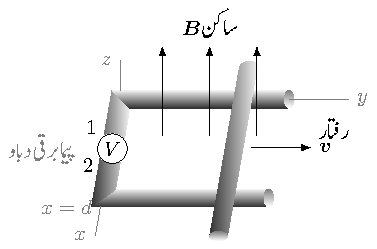
\includegraphics{figMaxwellSlidingConductorInStaticField}
\caption{وقت کے ساتھ نہ تبدیل ہوتے یکساں مقناطیسی میدان میں حرکت کرتے موصل سلاخ پر محرک برقی دباو پیدا ہوتی ہے۔}
\label{شکل_میکس_ویل_محرک_سلاخ_محرک_دباو}
\end{figure}

آئیں اب ایسی مثال دیکھیں جس میں وقت کے ساتھ تبدیل نہ ہونے والے مقناطیسی میدان میں  بند راہ حرکت کر رہی ہو۔شکل \حوالہ{شکل_میکس_ویل_محرک_سلاخ_محرک_دباو} میں ایسی صورت حال دکھائی گئی ہے۔اس شکل میں \عددیء{\kvec{v}} سمتی رفتار کو جبکہ \عددیء{V} برقی دباو ناپنے کی آلہ\حاشیہد{وولٹ میٹر} یعنی \اصطلاح{پیما برقی دباو}\فرہنگ{پیما!برقی دباو}\فرہنگ{برقی دباو!پیما}\حاشیہب{voltmeter}\فرہنگ{voltmeter} کو ظاہر کرتی ہے۔اس شکل میں دو افقی اور دو متوازی موصل سلاخ بند راہ یا بند دور بناتے ہیں۔ متوازی افقی سلاخوں کو بائیں طرف عمودی سلاخ سے جوڑا گیا ہے جس میں قابل نظر انداز جسامت اور لامحدود مزاحمت والا پیما برقی دباو نسب ہے، جبکہ دائیں جانب انہیں \عددیء{\kvec{v}} سمتی رفتار سے حرکت کرتے عمودی سلاخ سے جوڑا گیا ہے۔وقت کے ساتھ نہ تبدیل ہوتا اور ہر جگہ یکساں کثافت مقناطیسی بہاو \عددیء{\kvec{B}} بند راہ کی گھیرے سطح کے عمودی ہے۔

مثبت \عددیء{\kvec{B}} کی صورت میں \عددیء{\kvec{B}} کی سمت ہی بند راہ سے گھیری گئی سطح کی سمت ہو گی اور بند راہ کی سمت گھڑی کے الٹ ہو گی۔یوں راہ کے مثبت سمت میں دائیں ہاتھ کی انگلیاں رکھتے ہوئے گھیری سطح کی سمت انگوٹھے سے حاصل کی جاتی ہے۔ 

کسی بھی لمحہ \عددیء{t} پر حرکت کرتے سلاخ کے مقام کو \عددیء{y} سے ظاہر کرتے ہوئے ہم \عددیء{y=v t} لکھ سکتے ہیں جہاں \عددیء{v} سلاخ کے رفتار کی قیمت ہے۔یوں لمحہ \عددیء{t} پر بند دور کا ارتباط بہاو
\begin{align*}
\Phi=B d y =B d v t
\end{align*} 
ہو گا جو مساوات \حوالہ{مساوات_میکس_ویل_فیراڈے_قانون} کے تحت بند دور میں
\begin{align*}
e=-\frac{\dif \Phi}{\dif t}=-B d v
\end{align*}
محرک برقی دباو \عددیء{e} پیدا کرے گا۔

اب محرک برقی دباو \عددیء{\oint \kvec{E}\cdot \dif \kvec{L}} کو کہتے ہیں لہٰذا مندرجہ بالا جواب راہ پر گھڑی کے الٹ سمت میں اس بند لکیری تکمل سے بھی حاصل ہونا چاہیے۔ہم دیکھ چکے ہیں کہ برقی سکون کی صورت میں موصل کی سطح پر سطح کے متوازی \عددیء{E} صفر رہتی ہے۔ہم آگے دیکھیں گے کہ وقت کے ساتھ تبدیل ہوتے برقی میدان میں بھی موصل کی سطح پر متوازی \عددیء{E} صفر ہی رہتی ہے۔یوں شکل \حوالہ{شکل_میکس_ویل_محرک_سلاخ_محرک_دباو} پر گھڑی کے الٹ چلتے ہوئے تمام سلاخوں پر تکمل کی قیمت صفر کے برابر ہو گی۔پیما برقی دباو کی مزاحمت صفر نہیں ہے لہٰذا تکمل کی قیمت پیما برقی دباو پر مندرجہ بالا قیمت کے برابر ہونا ہو گا۔گھڑی کی الٹ سمت چلتے ہوئے پیما برقی دباو کی لمبائی کو \عددیء{\dif \kvec{L}} لکھتے ہوئے ہم دیکھتے ہیں کہ \عددیء{\kvec{E} \cdot \dif \kvec{L}=-B d v} ہونا ہو گا۔چونکہ \عددیء{\dif \kvec{L}=\dif L \ax} کے برابر ہے لہٰذا \عددیء{\kvec{E}} کی سمت \عددیء{\ax} کے الٹ ہو گی۔یوں پیما برقی دباو پر \عددیء{\kvec{E}} کی سمت پیما کے دوسرے سرے سے پہلے سرے کی جانب ہے اور پیما پر برقی دباو کا مثبت سرا پیما کا دوسرا سرا ہے۔

پیما کی جگہ مزاحمت جوڑنے سے دور میں گھڑی کے الٹ برقی رو گزرے گی جو \عددیء{\az} کے الٹ سمت میں مقناطیسی بہاو پیدا کرے گی۔یہ لورنز کے قانون کے عین مطابق ہے۔

آئیں اب اسی شکل میں دئے مسئلے کو حرکی برقی دباو تصور کرتے ہوئے حل کریں۔مقناطیسی میدان میں \عددیء{\kvec{v}} سمتی رفتار سے حرکت کرتے ہوئے چارج \عددیء{Q} پر قوت
\begin{align*}
\kvec{F}=Q \kvec{v} \times \kvec{B}
\end{align*}
یا حرکی شدت \عددیء{\kvec{E}_{\textrm{حرکی}}}
\begin{align}\label{مساوات_میکس_ویل_حرکی_برقی_شدت}
\kvec{E}_{\textrm{حرکی}}=\frac{\kvec{F}}{Q}=\kvec{v} \times \kvec{B}
\end{align}
عمل کرتی ہے۔حرکی شدت \عددیء{\ax} سمت میں ہے۔حرکت کرتے سلاخ میں ساکن مثبت ایٹم اور آزاد منفی الیکٹران پائے جاتے ہیں۔ان تمام چارجوں  پر ایسی قوت پائی جائے گی البتہ ساکن ایٹم مقید ہونے کی بنا حرکت نہیں کریں گے۔اگر محرک سلاخ کو متوازی سلاخوں سے اٹھایا جائے تو اس میں آزاد الیکٹران پر \عددیء{\ax} کے الٹ جانب قوت انہیں سلاخ کے پرلے سرے پر انبار کرنا شروع کر دے گی۔الیکٹرانوں کا انبار سلاخ میں \عددیء{-\ax} جانب برقی میدان کی شدت \عددیء{\kvec{E}_{\textrm{ساکن}}} پیدا کرے گا۔الیکٹران کا انبار بڑھتا رہے گا حتیٰ کہ  \عددیء{\kvec{E}_{\textrm{حرکی}}} اور \عددیء{\kvec{E}_{\textrm{ساکن}}} برابر ہو جائیں۔ایسا ہوتے ہی سلاخ میں کل برقی میدان کی شدت صفر ہو جائے گی اور اس میں چارج کا حرکت رک جائے گا۔

یوں حرکی برقی دباو
\begin{align}
\textrm{\RL{محرک برقی دباو}}=\oint \kvec{E}_{\textrm{حرکی}} \cdot \dif \kvec{L}=\oint \left(\kvec{v} \times \kvec{B} \right) \cdot \dif \kvec{L}
\end{align} 
سے حاصل ہو گی۔مساوات کے دائیں ہاتھ بند راہ کے ساکن حصوں پر تکمل کی قیمت صفر ہو گی لہٰذا محرک برقی دباو صرف حرکت کرتے حصوں کی وجہ سے پیدا ہو گی۔یوں حرکت کرتے سلاخ پر گھڑی کے الٹ چلتے ہوئے تکمل سے
\begin{align*}
\oint \left(\kvec{v} \times \kvec{B} \right) \cdot \dif \kvec{L}=\int_d^0 v B \dif x=-B v d
\end{align*}
حاصل ہوتا ہے ۔چونکہ \عددیء{\kvec{B}} اذ خود وقت کے ساتھ تبدیل نہیں ہو رہا لہٰذا یہی کل محرک برقی دباو ہو گا۔

یوں وقت کے ساتھ تبدیل نہ ہوتے مقناطیسی میدان میں حرکت کرتے بند راہ میں محرک برقی دباو حاصل کرتے وقت حرکت کرتے حصوں پر حرکی شدت \عددیء{\kvec{E}_{\textrm{حرکی}}} کے استعمال سے محرک برقی دباو یوں
\begin{align}
\textrm{\RL{محرک برقی دباو}}=\oint \kvec{E} \cdot \dif \kvec{L}=\oint \kvec{E}_{\textrm{حرکی}} \cdot \dif \kvec{L}=\oint \left(\kvec{v} \times \kvec{B} \right) \cdot \dif \kvec{L}
\end{align} 
حاصل کی جا سکتی ہے۔البتہ وقت کے ساتھ بدلتی مقناطیسی میدان میں محرک برقی دباو کے حصول میں مساوات \حوالہ{مساوات_میکس_ویل_پہلی_مساوات_تکمل_صورت} کا حصہ شامل کرنا ضروری ہے یوں محرک برقی دباو
\begin{align}
\textrm{\RL{محرک برقی دباو}}=\oint \kvec{E} \cdot \dif \kvec{L}=-\int_S \frac{\partial \kvec{B}}{\partial t} \cdot \dif \kvec{S}+\oint \left(\kvec{v} \times \kvec{B} \right) \cdot \dif \kvec{L}
\end{align} 
سے حاصل ہو گی۔یہ مساوات دراصل مساوات \حوالہ{مساوات_میکس_ویل_فیراڈے_قانون}
\begin{align*}
\textrm{\RL{محرک برقی دباو}}=-\frac{\dif \Phi}{\dif t}
\end{align*}
ہی ہے۔

\begin{figure}
\centering
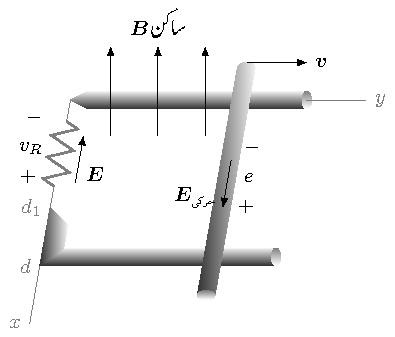
\includegraphics{figMaxwellDefiningElectromotiveForceEMF}
\caption{محرک برقی دباو اور برقی دباو کا موازنہ۔}
\label{شکل_میکس_ویل_محرک_دباو_اور_عام_دباو_موازنہ}
\end{figure}

آئیں شکل \حوالہ{شکل_میکس_ویل_محرک_سلاخ_محرک_دباو} میں پیما برقی دباو کی جگہ مزاحمت نسب کرتے ہوئے اس کی مدد سے  مساوات \حوالہ{مساوات_میکس_ویل_محرک_برقی_دباو_تعریف} جو محرک برقی دباو کی تعریف بیان کرتا ہے پر دوبارہ غور کریں۔نئی شکل کو شکل \حوالہ{شکل_میکس_ویل_محرک_دباو_اور_عام_دباو_موازنہ} میں دکھایا گیا ہے۔مساوات \حوالہ{مساوات_میکس_ویل_حرکی_برقی_شدت} محرک سلاخ پر پیدا \عددیء{\kvec{E}_{\textrm{حرکی}}} دیتا ہے جو سلاخ میں مثبت چارج کو سلاخ کے پرلے سرے کی طرف دھکیلے گا۔اس کے برعکس مزاحمت پر برقی دباو \عددیء{v_R} پایا جاتا ہے جس کی وجہ سے اس میں برقی میدان کی شدت \عددیء{\kvec{E}} پائی جائے گی جو مزاحمت میں مثبت چارج کو مزاحمت کے اُرلے سرے کی جانب دھکیلے گی۔

آپ شکل کو دیکھ کر تسلی کر لیں کہ مزاحمت پر میدان کی شدت \عددیء{\kvec{E}=E\ax} سے برقی دباو \عددیء{v_R} یوں
\begin{align}
v_R=-\int_d^0 \kvec{E} \cdot \dif \kvec{L}=-\int_d^0 E \dif x=Ed
\end{align}
حاصل ہوتی ہے جبکہ متحرک سلاخ پر حرکی شدت \عددیء{\kvec{E}_{\textrm{حرکی}}=-E_{\textrm{حرکی}}\ax} سے حرکی دباو \عددیء{e} یوں
\begin{align}
e=\oint \kvec{E}_{\textrm{حرکی}} \cdot \dif \kvec{L}=\int_d^0 \kvec{E}_{\textrm{حرکی}} \cdot \dif \kvec{L}=\int_d^0 -E_{\textrm{حرکی}} \dif x=E_{\textrm{حرکی}}d
\end{align}
حاصل ہوتی ہے۔یاد رہے کہ شکل میں \عددیء{v_R} اور \عددیء{e} دونوں مثبت قیمت رکھتے ہیں اور مثبت قیمتیں صرف مندرجہ بالا دو  مساوات سے ہی حاصل ہوتی ہیں۔یہاں ضرورت اس بات کی ہے کہ آپ دیکھ سکیں کہ \عددیء{v_R} کے حصول میں منفی کی علامت استعمال کی گئی جبکہ \عددیء{e} کے حصول میں ایسا نہیں کیا گیا۔حرکی دباو کے بند تکمل میں راہ کے بقایا اطراف پر تکمل کی قیمت صفر ہونے کے ناطے صرف متحرک سلاخ پر تکمل لیا گیا ہے۔


اگرچہ مساوات \حوالہ{مساوات_میکس_ویل_فیراڈے_قانون} انتہائی سادہ شکل رکھتی ہے لیکن اس کا استعمال کبھی کبھار مشکل ہو جاتا ہے۔ایسا اس وقت ہوتا ہے جب دور کے کسی حصے کو تبدیل کرتے ہوئے دوسرا حصہ نسب کیا جائے۔یہ بات شکل \حوالہ{شکل-میکس_ویل_سوئچ_سے_محرک_دباو_نہیں_پیدا_ہوتی} پر غور کرنے سے بہتر سمجھ آئے گی۔اس شکل میں نا تو وقت کے ساتھ تبدیل ہوتا مقناطیسی میدان ہے اور نا ہی بند راہ کا کوئی حصہ متحرک ہے۔البتہ شکل میں دکھائے سوئچ کو چالو یا غیر چالو کرتے ہوئے بند راہ میں مقناطیسی بہاو کم اور زیادہ کیا جا سکتا ہے۔یہاں بغیر سوچے مساوات \حوالہ{مساوات_میکس_ویل_فیراڈے_قانون} استعمال کرتے ہوئے غلط نتائج حاصل ہوتے ہیں۔ یاد رہے کہ برقی دباو یا تو وقت کے ساتھ بدلتے مقناطیسی میدان اور یا پھر بند راہ کے کسی حصے کے حرکت سے ہی پیدا ہو گا۔
  
\begin{figure}
\centering
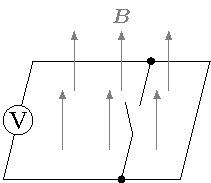
\includegraphics{figMaxwellSwitchingCoductorsToChangeFlux}
\caption{محرک برقی دباو یا تا وقت کے ساتھ بدلتی مقناطیسی میدان اور یا حرکت کرتے بند راہ سے ہی پیدا ہو سکتی ہے۔}
\label{شکل-میکس_ویل_سوئچ_سے_محرک_دباو_نہیں_پیدا_ہوتی}
\end{figure}

%==============
\ابتدا{مشق}
شکل \حوالہ{شکل-میکس_ویل_سوئچ_سے_محرک_دباو_نہیں_پیدا_ہوتی} میں \عددیء{\kvec{B}=0.5\az } ٹسلا، رفتار \عددیء{100 y \ay} میٹر فی سیکنڈ جبکہ \عددیء{d=0.5} میٹر ہے۔اگر \عددیء{t=0} پر \عددیء{y=0.2} میٹر ہو تب \عددیء{t=15} ملی سیکنڈ پر مندرجہ ذیل حاصل کریں۔
\begin{itemize}
\item
سلاخ کی رفتار،
\item
محرک برقی دباو \عددیء{V_{21}}،
\item
پیما برقی دباو کی اندرونی مزاحمت دس میگا اوہم کی صورت میں دور میں برقی رو۔
\end{itemize} 

جوابات:\عددیء{\SI{4.017}{\meter\per\second}}، \عددیء{\SI{100}{\volt}}، \عددیء{\SI{10}{\micro \ampere}}

\انتہا{مشق}
%=======================

\حصہ{انتقالی برقی رو}
فیراڈے کے تجرباتی نتیجے سے میکس ویل کی پہلی مساوات
\begin{align}\label{مساوات_میکس_ویل_انتقالی_رو_الف}
\nabla \times \kvec{E}=-\frac{\partial \kvec{B}}{\partial t}
\end{align}
حاصل ہوئی جو کہتا ہے کہ بدلتی مقناطیسی میدان پیدا کرتا ہے برقی دباو۔گردش کے عمل کو مد نظر رکھتے ہوئے ہم دیکھتے ہیں ایسے پیدا کردہ برقی دباو کا بند لکیری تکمل صفر کے برابر نہیں ہوتا۔ آئیں اب وقت کے ساتھ تبدیل ہوتے برقی میدان پر غور کریں۔

ایمپیئر کے دوری قانون کی نقطہ شکل
\begin{align}\label{مساوات_میکس_ویل_ایمپیئر_دوری_نقطہ_صورت}
\nabla \times \kvec{H}=\kvec{J}
\end{align}
ساکن مقناطیسی میدان پر لاگو ہوتی ہے۔اس مساوات کی پھیلاو
\begin{align*}
\nabla \cdot \nabla \times \kvec{H}=0=\nabla \cdot \kvec{J}
\end{align*}
 لیتے ہوئے ہم دیکھتے ہیں کہ گردش کی پھیلاو ہر صورت صفر کے برابر ہوتی ہے لہٰذا مندرجہ بالا مساوات کا بایاں ہاتھ ہر صورت صفر دے گا اور یوں اگر یہ مساوات درست ہو تب اس کا دایاں ہاتھ بھی ہر صورت صفر ہونا چاہیے۔مگر ہم استمراری  مساوات سے جانتے ہیں کہ
\begin{align}
\nabla \cdot \kvec{J}=-\frac{\partial \rho}{\partial t}
\end{align} 
ہوتا ہے۔اس سے ثابت ہوتا ہے کہ مساوات \حوالہ{مساوات_میکس_ویل_ایمپیئر_دوری_نقطہ_صورت} صرف اس صورت درست ہو گا جب \عددیء{\tfrac{\partial \rho}{\partial t}=0} ہو۔یہ ایک غیر ضروری اور غیر حقیقی شرط ہے لہٰذا وقت کے ساتھ تبدیل ہوتے برقی میدان پر استعمال کے قابل بنانے کی خاطر  مساوات \حوالہ{مساوات_میکس_ویل_ایمپیئر_دوری_نقطہ_صورت} کو تبدیل کرنا لازم ہے۔تصور کریں کہ مساوات \حوالہ{مساوات_میکس_ویل_ایمپیئر_دوری_نقطہ_صورت} میں نا معلوم جزو \عددیء{\kvec{G}} کی شمولیت سے یہ مساوات وقت  کے ساتھ تبدیل ہوتے برقی میدان پر بھی لاگو کرنے کے قابل ہو جاتا ہے۔ایسی صورت میں مساوات \حوالہ{مساوات_میکس_ویل_ایمپیئر_دوری_نقطہ_صورت} یوں
\begin{align*}
\nabla \times \kvec{H}=\kvec{J}+\kvec{G}
\end{align*}
لکھی جائے گی۔آئیں دوبارہ اس کی پھیلاو حاصل کریں جس سے
\begin{align*}
0=\nabla \cdot \kvec{J}+\nabla \cdot \kvec{G}
\end{align*}
یا
\begin{align*}
\nabla \cdot \kvec{G}=\frac{\partial \rho}{\partial t}
\end{align*}
حاصل ہوتا ہے جہاں استمراری مساوات کا سہارا لیا گیا۔اس مساوات میں \عددیء{\rho} کی جگہ \عددیء{\nabla \cdot \kvec{D}} پر کرنے سے
\begin{align*}
\nabla \cdot \kvec{G}=\frac{\partial \left(\nabla \cdot \kvec{D} \right)}{\partial t}=\nabla \cdot \frac{\partial \kvec{D}}{\partial t}
\end{align*}
یعنی
 \begin{align*}
\kvec{G}=\frac{\partial \kvec{D}}{\partial t}
\end{align*}
حاصل ہوتا ہے۔یوں ایمپیئر کے دوری قانون کی درست شکل
\begin{align}\label{مساوات-میکس_ویل_دوسری_مساوات_نقطہ_شکل}
\nabla \times \kvec{H}=\kvec{J}+\frac{\partial \kvec{D}}{\partial t}
\end{align}
ہے۔ مندرجہ بالا مساوات برقی و مقناطیسیات کے اب تک تمام دریافت کردہ اصولوں پر پورا اترتی آئی ہے۔جب تک یہ غلط ثابت نہ ہو جائے، ہم اسے درست ہی تصور کریں گے۔

مساوات \حوالہ{مساوات-میکس_ویل_دوسری_مساوات_نقطہ_شکل} میکس ویل کے مساوات میں سے ایک مساوات ہے۔اس مساوات میں \عددیء{\tfrac{\partial \kvec{D}}{\partial t}} کی بُعد ایمپیئر فی مربع میٹر حاصل ہوتی ہے جو کثافت برقی رو کا بُعد ہے۔میکس ویل نے اس مساوات میں دائیں ہاتھ نئے جزو  کو \اصطلاح{کثافت انتقالی رو}\فرہنگ{کثافت!انتقالی رو}\فرہنگ{رو!کثافت انتقالی}\حاشیہب{displacement current density}\فرہنگ{displacement current density}\فرہنگ{current!displacement} کا نام دیا اور \عددیء{\kvec{J}_d} سے ظاہر کیا یعنی
\begin{align*}
\nabla \times \kvec{H}&=\kvec{J}+\kvec{J}_d\\
\kvec{J}_d&=\frac{\partial \kvec{D}}{\partial t}
\end{align*}

ہم تین اقسام کے کثافت رو دیکھ چکے جن میں کثافت انتقالی رو\فرہنگ{رو!انتقالی} کے علاوہ  غیر چارج شدہ خطے میں عموماً الیکٹران کے حرکت سے پیدا  کثافت ایصالی رو\فرہنگ{رو!ایصالی}
\begin{align}
\kvec{J}=\sigma \kvec{E}
\end{align}
اور چارج کے حجم کے حرکت سے پیدا کثافت اتصالی رو\فرہنگ{رو!اتصالی}
\begin{align}
\kvec{J}=\rho_h \kvec{v}
\end{align}
شامل ہیں۔مساوات \حوالہ{مساوات-میکس_ویل_دوسری_مساوات_نقطہ_شکل} میں \عددیء{\kvec{J}} سے مراد ایصالی اور اتصالی رو کے کثافتوں کا مجموعہ ہے جبکہ مقید چارج \عددیء{\kvec{H}} کا حصہ ہیں۔غیر موصل خطے میں جہاں کثافت چارج پائی ہی نہیں جاتی \عددیء{\kvec{J}=0} ہوتا ہے لہٰذا غیر موصل میں
\begin{align}\label{مساوات_میکس_ویل_مقناطیسی_شدت_گردش}
\nabla \times \kvec{H}=\frac{\partial \kvec{D}}{\partial t}  \quad \quad (\kvec{J}=0)
\end{align}
ہو گا۔مساوات \حوالہ{مساوات_میکس_ویل_مقناطیسی_شدت_گردش} اور مساوات \حوالہ{مساوات_میکس_ویل_انتقالی_رو_الف} میں مشابہت دیکھیں۔
\begin{align*}
\nabla \times \kvec{E}=-\frac{\partial \kvec{B}}{\partial t}
\end{align*} 
مقناطیسی شدت \عددیء{\kvec{H}} اور برقی شدت \عددیء{\kvec{E}} کافی مشابہت رکھتے ہیں۔ اسی طرح کثافت رو \عددیء{\kvec{D}} اور کثافت بہاو \عددیء{\kvec{B}} بھی کافی مشابہت رکھتے ہیں۔اس مشابہت کو یہیں تک رکھیں چونکہ جیسے ہی میدان میں چارج پر قوت کی بات کی جائے، دونوں اقسام کے میدان بالکل مختلف طریقوں سے  عمل کرتے ہیں۔

کسی بھی سطح سے کل انتقالی رو سطحی تکمل
\begin{align}
I_d=\int_S \kvec{J}_d \cdot \dif \kvec{S}=\int_S \frac{\partial \kvec{D}}{\partial t} \cdot \dif \kvec{S}
\end{align}
سے حاصل ہو گی۔مساوات \حوالہ{مساوات-میکس_ویل_دوسری_مساوات_نقطہ_شکل} کے سطحی تکمل
\begin{align*}
\int_S \left(\nabla \times \kvec{H} \right) \cdot \dif \kvec{S}=\int_S \kvec{J} \cdot \dif \kvec{S}+\int_S \frac{\partial \kvec{D}}{\partial t} \cdot \dif \kvec{S}
\end{align*}
پر مسئلہ سٹوکس کے اطلاق سے
\begin{align}
\oint \kvec{H} \cdot \dif \kvec{L}=I+I_d=I+\int_S \frac{\partial \kvec{D}}{\partial t} \cdot \dif \kvec{S}
\end{align}
 وقت کے ساتھ تبدیل ہوتے ایمپیئر کے دوری قانون\فرہنگ{ایمپیئر قانون!عمومی نقطہ شکل} کی نقطہ شکل حاصل ہوتی ہے۔

\begin{figure}
\centering
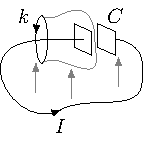
\includegraphics{figMaxwellConductionDisplacementCurrents}
\caption{موصل تار میں ایصالی رو کپیسٹر کے چادروں کے درمیان انتقالی رو کے برابر ہے۔}
\label{شکل_میکس_ویل_ایصالی_انتقالی_رو}
\end{figure}

انتقالی رو کو شکل \حوالہ{شکل_میکس_ویل_ایصالی_انتقالی_رو} کی مدد سے سمجھتے ہیں جہاں موصل تار سے کپیسٹر \عددیء{C} کے دو سرے جوڑتے ہوئے بند دور بنایا گیا ہے جس میں وقت کے ساتھ بدلتی سائن نما مقناطیسی میدان \عددیء{\kvec{B}} محرک برقی دباو
\begin{align*}
e=V_0 \cos \omega t
\end{align*}
 پیدا کرتی ہے۔یہ سادہ برقی دور ہے جس میں مزاحمت اور امالہ کو نظر انداز کرتے ہوئے برقی رو
\begin{align*}
i&=-\omega C V_0 \sin \omega t\\
&=-\omega \frac{\epsilon S}{d} V_0 \sin \omega t
\end{align*}
لکھی جا سکتی ہے جہاں \عددیء{\epsilon}، \عددیء{S} اور \عددیء{d} کپیسٹر سے متعلق ہیں۔آئیں انتقالی رو کو نظرانداز کرتے ہوئے تار کے گرد بند راہ  \عددیء{k} پر ایمپیئر کا دوری قانون لاگو کریں۔
\begin{align*}
\oint_k \kvec{H} \cdot \dif \kvec{L}=I_k
\end{align*}
اب بند راہ \عددیء{k} اور اس راہ پر \عددیء{\kvec{H}} حقیقی مقدار ہیں اور تکمل سے حاصل رو \عددیء{I_k} اس راہ سے گھیرے کسی بھی سطح سے گزرتی رو کو ظاہر کرتی ہے۔اگر ہم \عددیء{k} کو سیدھی سطح کا سرحد تصور کریں تب موصل تار اس سطح کو چھیدتا ہوا گزرے گا۔یوں اس سطح سے \عددیء{I} رو ہی گزرے گی جو ایصالی رو ہے۔اس کے برعکس اگر ہم \عددیء{k} کو تھیلے کا منہ تصور کریں جیسے شکل میں دکھایا گیا ہے تب ایصالی رو ایسی سطح سے نہیں گزرتی چونکہ تھیلا کپیسٹر کے دو چادروں کے درمیان سے گزرتا ہے اور تار اسے چھوتی تک نہیں۔ایسی صورت میں تھیلے سے گزرتی ایصالی رو صفر کے برابر ہے۔ایسی صورت میں ہمیں انتقالی رو کا سہارا لینا ہو گا۔کپیسٹر کے چادروں کے درمیان
\begin{align*}
D=\epsilon E=\epsilon \left(\frac{V_0}{d} \cos \omega t \right)
\end{align*}
ہے لہٰذا
\begin{align*}
J_d=\frac{\partial D}{\partial t}=-\omega \epsilon \frac{V_0}{d} \sin \omega t
\end{align*}
اور یوں
\begin{align*}
I_d=S J_d =-\omega \frac{\epsilon  S}{d} V_0\sin \omega t 
\end{align*}
ہو گی۔

یہ وہی جواب ہے جو ایصالی رو سے حاصل ہوا تھا۔اس مثال سے آپ دیکھ سکتے ہیں کہ ایمپیئر کے دوری قانون کو استعمال کرتے ہوئے سطح سے  گزرتی ایصالی رو اور انتقالی رو دونوں کا خیال رکھنا ہو گا۔کہیں پر سطح سے صرف ایصالی رو گزرے گی تو کہیں اس سے صرف انتقالی رو گزرے گی اور کبھی کبھار دونوں کا مجموعہ۔

انتقالی رو وقت کے ساتھ بدلتے برقی میدان سے پیدا ہوتے ہیں لہٰذا یہ ایسے تمام غیر موصل یا نیم موصل خطوں میں پائی جاتی ہے جہاں وقت کے ساتھ تبدیل ہوتی ایصالی رو پائی جائے۔اگرچہ موصل خطے میں بھی انتقالی رو پائی جاتی ہے لیکن، جیسے آپ مندرجہ ذیل مشق میں دیکھیں گے، اس کی قیمت ایصالی رو کی نسبت سے اتنی کم ہوتی ہے کہ یہ قابل نظر انداز ہوتی ہے۔یہی وجہ ہے کہ انتقالی رو تجرباتی طور دریافت نہیں کی گئی بلکہ اس تک منطق کے ذریعہ سے پہنچا گیا۔

%=====================
\ابتدا{مشق}
ٹھوس تانبے کی تار میں سائن نما، پچاس ہرٹز کی ایصالی رو \عددیء{I_0 \cos \omega t} گزر رہی ہے۔اس میں انتقالی رو حاصل کریں۔پچاس ہرٹز رو کی صورت میں ایصالی اور انتقالی رو کے موثر قیمت کی شرح حاصل کریں۔

حل:\عددیء{I_d=-\tfrac{\omega \epsilon_0}{\sigma} I_0\sin \omega t} جبکہ ان کے موثر قیمت کی شرح  \عددیء{\tfrac{I}{I_d}=\tfrac{\sigma}{\omega \epsilon_0}=\num{2.08e16}} ہے۔

\انتہا{مشق}
%====================

\حصہ{میکس ویل مساوات کی نقطہ شکل}
ہم وقت کے ساتھ تبدیل ہوتے میدانوں میں میکس ویل کے دو مساوات کے نقطہ اشکال\فرہنگ{میکس ویل!نقطہ اشکال}\فرہنگ{Maxwell's equation!point form}
\begin{align}\label{مساوات-میکس_ویل_تفرقی_الف}
\nabla \times \kvec{E}=-\frac{\partial \kvec{B}}{\partial t}
\end{align}
اور
\begin{align}\label{مساوات-میکس_ویل_تفرقی_ب}
\nabla \times \kvec{H}=\kvec{J}+\frac{\partial \kvec{D}}{\partial t}
\end{align}
 حاصل کر چکے ہیں۔میکس ویل کے بقایا دو مساوات وقت کے ساتھ تبدیل ہوتے میدان میں بھی جوں کے توں
\begin{align}
\nabla \cdot \kvec{D}&=\rho_h \label{مساوات_میکس_ویل_گاوس_قانون_نقطہ}\\
\nabla \cdot \kvec{B}&=0 \label{مساوات_میکس_ویل_مقناطیسی_میدان_دو_قطب}
\end{align}
 رہتے ہیں۔ 

مساوات \حوالہ{مساوات_میکس_ویل_گاوس_قانون_نقطہ} کہتا ہے کہ کثافت برقی رو کا منبع کثافت چارج  ہے۔وقت کے ساتھ بدلتے مقناطیسی میدان میں برقی میدان  پیدا ہوتا ہے جو بند راہ پر چلتا ہے۔ایسے برقی میدان کا نا تو کسی چارج سے اخراج ہوتا ہے اور نا ہی یہ کسی چارج پر ختم ہوتا ہے۔اس کے برعکس ہر مثبت چارج سے اس کے برابر برقی بہاو کا اخراج ہوتا ہے اور ہر منفی چارج پر اس کے برابر برقی بہاو کا اختتام ہوتا ہے۔
  

مساوات \حوالہ{مساوات_میکس_ویل_مقناطیسی_میدان_دو_قطب} کہتا ہے کہ کسی بھی نقطے سے کل مقناطیسی بہاو کا اخراج صفر ہے یعنی مقناطیسی بہاو نا تو کسی نقطے سے خارج ہوتا ہے اور نا ہی یہ کسی نقطے پر اختتام پذیر ہوتا ہے۔ سادہ زبان میں اس کا مطلب ہے کہ مقناطیس کا یک قطب ممکن نہیں جس سے مقناطیسی بہاو کا اخراج ہو یا اس پر مقناطیسی بہاو اختتام ہو۔

مندرجہ بالا چار مساوات پر برقی و مقناطیسیات کی بنیاد کھڑی ہے جنہیں استعمال کرنے کی خاطر چار معاون مساوات
\begin{align}
\kvec{D}&=\epsilon \kvec{E} \label{مساوات_میکس_ویل_خالی_خلاء_برقی_مستقل}\\
\kvec{B}&=\mu \kvec{H} \label{مساوات_میکس_ویل_خالی_خلاء_مقناطیسی_مستقل}\\
\kvec{J}&=\sigma \kvec{E}\\
\kvec{J}&=\rho_h \kvec{v}
\end{align}
بھی درکار ہوتے ہیں۔

ایسے ذو برق اور مقناطیسی اشیاء جن میں متغیرات سادہ تعلق نہ رکھتے ہوں، ان میں مساوات \حوالہ{مساوات_میکس_ویل_خالی_خلاء_برقی_مستقل} اور مساوات \حوالہ{مساوات_میکس_ویل_خالی_خلاء_مقناطیسی_مستقل} کی جگہ
\begin{align}
\kvec{D}&=\epsilon_0 \kvec{E}+\kvec{P}\\
\kvec{B}&=\mu_0 \left(\kvec{H}+\kvec{M} \right)
\end{align}
استعمال ہوتے ہیں۔خطی اشیاء میں
\begin{align}
\kvec{P}=\chi_e \kvec{E}
\end{align}
اور
\begin{align}
\kvec{M}=\chi_m \kvec{H}
\end{align}
لکھا جا سکتا ہے۔

آخر میں لورنز قوت کی مساوات 
\begin{align}
\kvec{F}=\rho_h \left(\kvec{E}+\kvec{v} \times \kvec{B} \right)
\end{align}
بھی شامل کرتے ہیں۔

غیر سمتی مقناطیسی دباو \عددیء{V} اور سمتی مقناطیسی دباو \عددیء{\kvec{A}} انتہائی اہم ہیں البتہ ان کی شمولیت لازم نہیں۔

\حصہ{میکس ویل مساوات کی تکمل شکل}
 مساوات \حوالہ{مساوات-میکس_ویل_تفرقی_الف} کے سطحی تکمل پر مسئلہ سٹوکس کا اطلاق کرتے ہوئے فیراڈے کا قانون
\begin{align}\label{مساوات_میکس_ویل_تکمل_مساوات_الف}
\oint \kvec{E} \cdot \dif \kvec{L}=-\int_S \frac{\partial \kvec{B}}{\partial t} \cdot \kvec{S}
\end{align}
حاصل ہوتا ہے۔اسی طرح مساوات \حوالہ{مساوات-میکس_ویل_تفرقی_ب} اسی طریقہ کار سے ایمپیئر کا دوری قانون
\begin{align}\label{مساوات_میکس_ویل_تکمل_مساوات_ب}
\oint \kvec{H} \cdot \dif \kvec{L}=I+\int_S \frac{\partial \kvec{D}}{\partial t} \cdot \dif \kvec{S}
\end{align}
حاصل ہوتا ہے۔

برقی اور مقناطیسی میدان کے لئے گاؤس کے قوانین مساوات \حوالہ{مساوات_میکس_ویل_گاوس_قانون_نقطہ} اور مساوات \حوالہ{مساوات_میکس_ویل_مقناطیسی_میدان_دو_قطب} کے تمام حجم پر حجمی تکمل اور مسئلہ پھیلاو کی مدد سے 
\begin{align}\label{مساوات_میکس_ویل_تکمل_مساوات_پ}
\oint_S \kvec{D} \cdot \dif \kvec{S}=\int_h \rho_h \dif h
\end{align}
اور
\begin{align}\label{مساوات_میکس_ویل_تکمل_مساوات_ت}
\oint_S \kvec{B} \cdot \dif \kvec{S}=0
\end{align}
حاصل ہوتے ہیں۔

مندرجہ بالا چار مساوات سے \عددیء{\kvec{E}}، \عددیء{\kvec{H}}، \عددیء{\kvec{D}} اور \عددیء{\kvec{B}} کے سرحدی شرائط حاصل ہوتے ہیں جن سے میکس ویل کے جزوی تفرقی مساوات کے مستقل حاصل کئے جاتے ہیں۔وقت کے ساتھ تبدیل ہوتے میدان کے سرحدی شرائط عموماً ساکن میدان کے سرحدی شرائط ہی ہوتے ہیں لہٰذا ساکن میدان کے طریقہ کار سے وقت کے ساتھ بدلتے میدان کے سرحدی شرائط بھی حاصل کئے جا سکتے ہیں۔

\begin{figure}
\centering
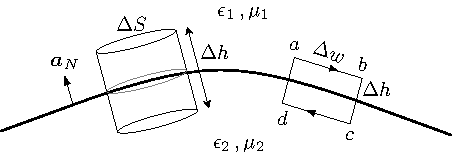
\includegraphics{figMaxwellBoundaryConditions}
\caption{وقت کے ساتھ بدلتے میدان کے سرحدی شرائط۔}
\label{شکل_میکس_ویل_سرحدی_شرائط}
\end{figure}

آئیں شکل \حوالہ{شکل_میکس_ویل_سرحدی_شرائط}  کی مدد سے  سرحد کے متوازی برقی اور مقناطیسی شرائط\فرہنگ{سرحدی شرائط!برقی اور مقناطیسی}\فرہنگ{برقی میدان!سرحدی شرائط}\فرہنگ{مقناطیسی میدان!سرحدی شرائط}\فرہنگ{boundary conditions! electric and magnetic}\فرہنگ{electric field!boundary conditions}\فرہنگ{magnetic field!boundary conditions} حاصل کریں۔ شکل میں مستطیل راہ پر مساوات \حوالہ{مساوات_میکس_ویل_تکمل_مساوات_الف} کے اطلاق سے
\begin{align*}
\left(E_{m1}-E_{m2}\right) \Delta w=-\frac{\partial B_{n}}{\partial t}  \Delta w \Delta h
\end{align*}  
لکھا جا سکتا ہے جہاں \عددیء{\tfrac{\partial B_{n}}{\partial t}} سے مراد راہ کے گھیرے سطح سے گزرتی مجموعی میدان کی تبدیلی ہے جس کا کچھ حصہ خطہ \عددیء{1} اور کچھ حصہ خطہ \عددیء{2} سے گزرتا ہے۔اس مساوات کے دائیں ہاتھ کی قیمت \عددیء{\Delta h \to 0} کرتے ہوئے صفر کے قریب تر کی جا سکتی ہے۔ایسی صورت میں دائیں ہاتھ کو صفر ہی تصور کرتے ہوئے
\begin{align}\label{مساوات_میکس_ویل_سرحدی_شرائط_بدلتے_میدان_الف}
E_{m1}=E_{m2}
\end{align}
یعنی
\begin{align}
\aN \times \left(\kvec{E}_1-\kvec{E}_2 \right)=0
\end{align}
حاصل ہوتا ہے۔

سرحد پر انتہائی کم موٹائی کے خطے میں کثافت برقی رو \عددیء{\kvec{K}} تصور کرتے ہوئے کسی بھی چھوٹی لمبائی \عددیء{\dif \kvec{L}} پر برقی رو کو \عددیء{I=\kvec{K} \cdot \dif \kvec{L}} لکھی جا سکتی ہے۔یوں شکل \حوالہ{شکل_میکس_ویل_سرحدی_شرائط} میں مستطیل راہ پر مساوات \حوالہ{مساوات_میکس_ویل_تکمل_مساوات_پ} کے اطلاق سے
\begin{align*}
\left(H_{m1}-H_{m2} \right) \Delta w=K_\perp \Delta w +\frac{\partial D}{\partial t} \Delta w \Delta h
\end{align*}
حاصل ہوتا ہے جہاں \عددیء{K_\perp} سے مراد \عددیء{K} کا وہ حصہ ہے جو \عددیء{H_{m1}} اور \عددیء{H_{m2}} کے عمودی ہے۔دائیں ہاتھ دوسرے جزو کی قیمت \عددیء{\Delta h \to 0} کرتے ہوئے صفر کے قریب تر کی جا سکتی ہے لہٰذا اس جزو کو نظرانداز کرتے ہوئے
\begin{align}
H_{m1}-H_{m2}=K_\perp
\end{align}
حاصل ہوتا ہے جسے یوں
\begin{align}
\aN \times \left(\kvec{H}_1-\kvec{H}_2 \right)=\kvec{K}_\perp
\end{align}
بھی لکھا جا سکتا ہے۔

کسی بھی حقیقی دو مختلف اشیاء کے سرحد، مثلاً سمندر کے پانی اور ہوا کے سرحد یا ہوا اور دیوار کے سرحد، پر کثافت برقی رو \عددیء{\kvec{K}} صفر ہوتی ہے۔لہٰذا حقیقی مسائل میں \عددیء{K=0} کی بنا پر
\begin{align}\label{مساوات_میکس_ویل_سرحدی_شرائط_بدلتے_میدان_ب}
H_{m1}=H_{m2}
\end{align}
ہو گا۔صفحہ \حوالہصفحہ{شکل_امالہ_مقناطیسی_سرحدی_شرائط} پر شکل \حوالہ{شکل_امالہ_مقناطیسی_سرحدی_شرائط} میں سطحی کثافت برقی رو \عددیء{\kvec{K}} دکھائی گئی ہے جبکہ یہاں شکل \حوالہ{شکل_میکس_ویل_سرحدی_شرائط} میں اسے صفر تصور کرتے ہوئے نہیں دکھایا گیا۔

مساوات \حوالہ{مساوات_میکس_ویل_تکمل_مساوات_پ} اور مساوات \حوالہ{مساوات_میکس_ویل_تکمل_مساوات_ت} سے سرحدی عمودی شرائط
\begin{align}\label{مساوات_میکس_ویل_سرحدی_شرائط_بدلتے_میدان_پ}
\aN \cdot \left(\kvec{D}_1-\kvec{D}_2 \right)&=\rho_S
\end{align}
اور
\begin{align}\label{مساوات_میکس_ویل_سرحدی_شرائط_بدلتے_میدان_ت}
\aN \cdot \left(\kvec{B}_1-\kvec{B}_2 \right)=0
\end{align}
حاصل ہوتے ہیں۔

موصل کو ایسا کامل موصل تصور کرتے ہوئے جس کی موصلیت لامحدود مگر \عددیء{\kvec{J}} محدود ہو سے موصل کے اندر اوہم کے قانون سے
\begin{align}
\kvec{E}=0
\end{align}
اور یوں فیراڈے کے قانون کی نقطہ شکل سے، وقت کے ساتھ تبدیل ہوتے میدان کی صورت میں
\begin{align}
\kvec{H}=0
\end{align}
حاصل ہوتے ہیں۔اس طرح ایمپیئر کے دوری قانون کی نقطہ شکل سے محدود \عددیء{\kvec{J}} کی قیمت
\begin{align}
\kvec{J}=0
\end{align}
حاصل ہوتی ہے لہٰذا برقی رو صرف موصل کی سطح پر بطور سطحی کثافت رو \عددیء{\kvec{K}} ممکن ہے۔یوں اگر خطہ \عددیء{2} کامل موصل ہو تب مساوات \حوالہ{مساوات_میکس_ویل_سرحدی_شرائط_بدلتے_میدان_الف} تا مساوات \حوالہ{مساوات_میکس_ویل_سرحدی_شرائط_بدلتے_میدان_ت} سے
\begin{align}
E_{m1}&=0   \label{مساوات_میکس_ویل_کامل_موصل_سرحدی_شرط_الف}\\
H_{m1}&=0   \label{مساوات_میکس_ویل_کامل_موصل_سرحدی_شرط_ب}\\
D_{n1}&=\rho_S    \label{مساوات_میکس_ویل_کامل_موصل_سرحدی_شرط_پ}\\
B_{n1}&=0    \label{مساوات_میکس_ویل_کامل_موصل_سرحدی_شرط_ت}
\end{align}
حاصل ہوتے ہیں۔یاد رہے کہ سطحی کثافت چارج کی موجودگی ذو برق، کامل موصل اور غیر کامل موصل تمام پر ممکن ہے جبکہ سطحی کثافت رو \عددیء{\kvec{K}} صرف کامل موصل کی صورت میں ممکن ہے۔

مندرجہ بالا سرحدی شرائط میکس ویل کے مساوات کے حل کے لئے لازم  ہیں۔حقیقت میں پیش آنے والے تمام مسائل میں مختلف اشیاء کے سرحدیں پائی جاتی ہیں اور ایسے ہر سرحد کے دونوں اطراف پر مختلف متغیرات کے تعلق سرحدی شرائط سے ہی حاصل کرنا ممکن ہے۔کامل موصل کی صورت میں موصل کے اندر،  وقت کے ساتھ بدلتے، تمام متغیرات صفر ہوتے ہیں البتہ ایسی صورت میں مساوات \حوالہ{مساوات_میکس_ویل_کامل_موصل_سرحدی_شرط_الف} تا مساوات \حوالہ{مساوات_میکس_ویل_کامل_موصل_سرحدی_شرط_ت} میں دئے شرائط کا اطلاق نہایت مشکل ہوتا ہے۔

متحرک لہروں کے چند بنیادی خاصیت بغیر سرحد کے خطے میں لہر کی حرکت پر غور سے واضح ہوتے ہیں۔اگلا باب انہیں متحرک لہروں پر ہے۔میکس ویل مساوات کا یہ سب سے آسان استعمال ہے چونکہ ان میں کسی قسم کے سرحدی شرائط لاگو نہیں ہوتے۔ 


\حصہ{تاخیری دباو}
وقت کے ساتھ بدلتے دباو، جنہیں \اصطلاح{تاخیری دباو}\فرہنگ{تاخیری دباو}\حاشیہب{retarded potentials}\فرہنگ{retarded potentials} کہا جاتا ہے، \اصطلاح{اشعاعی اخراج}\فرہنگ{اشعاعی اخراج}\حاشیہب{radiation}\فرہنگ{radiation}  کے مسائل حل کرنے میں نہایت اہم ثابت ہوتے ہیں۔آپ کو یاد ہو گا کہ غیر سمتی مقناطیسی دباو \عددیء{V} کو خطے میں تقسیم ساکن چارج کی صورت
\begin{align}\label{مساوات_میکس_ویل_بدلتا_میدان_غیر_سمتی_دباو}
V=\int_h \frac{\rho_h \dif  h}{4 \pi \epsilon R} \quad \quad (\textrm{\RL{برقی سکون}})
\end{align}
میں لکھا جا سکتا ہے۔اسی طرح سمتی مقناطیسی دباو \عددیء{\kvec{A}} کو وقت کے ساتھ نہ بدلتے یعنی یک سمتی برقی رو کے تقسیم کی صورت
\begin{align}\label{مساوات_میکس_ویل_بدلتا_میدان_سمتی_دباو}
\kvec{A}=\int_h \frac{\mu \kvec{J} \dif h}{4\pi R} \quad \quad (\textrm{\RL{یک سمتی رو}})
\end{align}
میں لکھا جا سکتا ہے۔انہیں مساوات کے نقطہ اشکال بالترتیب
\begin{align}\label{مساوات_میکس-ویل_بدلتا_میدان_مساوات_الف}
\nabla^2 V=-\frac{\rho_h}{\epsilon}  \quad \quad (\textrm{\RL{برقی سکون}})
\end{align}
اور
\begin{align}\label{مساوات_میکس-ویل_بدلتا_میدان_مساوات_ب}
\nabla^2 \kvec{A}=-\mu \kvec{J}   \quad \quad (\textrm{\RL{یک سمتی رو}})
\end{align}
ہیں۔

غیر سمتی اور سمتی مقناطیسی دباو کے حصول کے بعد میدان کے بنیادی متغیرات ڈھلوان
\begin{align}\label{مساوات_میکس-ویل_بدلتا_میدان_مساوات_پ}
\kvec{E}=-\nabla V  \quad \quad (\textrm{\RL{برقی سکون}})
\end{align}
اور گردش
\begin{align}\label{مساوات_میکس-ویل_بدلتا_میدان_مساوات_ت}
\kvec{B}=\nabla \times \kvec{A}   \quad \quad (\textrm{\RL{یک سمتی رو}})
\end{align}
کی مدد سے حاصل ہوتے ہیں۔

آئیں اب ساکن چارج اور یک سمتی رو سے متعلق، وقت کے ساتھ تبدیل ہوتے ایسے دباو حاصل کریں جو مندرجہ بالا مساوات پر پورا اترتے ہوں۔

میکس ویل کے مساوات کے تحت \عددیء{\nabla \cdot \kvec{B}=0} ہو گا۔مساوات \حوالہ{مساوات_میکس-ویل_بدلتا_میدان_مساوات_ت} اس شرط پر پورا اترتی ہے چونکہ گردش کی پھیلاو لازماً صفر کے برابر ہی ہوتی ہے۔یوں مساوات \حوالہ{مساوات_میکس-ویل_بدلتا_میدان_مساوات_ت} کو بدلتے میدان کے لئے بھی درست تصور کرتے ہیں۔
